%!TEX root =  ../main.tex


\objective{Utilize standard angle values and circular symmetry}


There are not many angles we could draw for which we could precisely name
the displacement involved.  Two shapes we know every such thing about are the 
square and the equilateral triangle.  We might begin by drawing a square with
sides of length 1, and then drawing a diagonal.

\begin{figure}[h]
\begin{center}
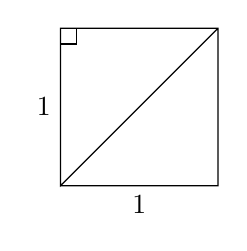
\begin{tikzpicture}[scale=2]
	\draw (0,0) -- (1,0) -- (1,1) -- (0,1) -- (0,0) -- (1,1);
	\draw (0,0.9) -- (.1,.9) -- (.1,1);
	\node at (0.5,0) [anchor=north] {1};
	\node at (0,0.5) [anchor=east] {1};
\end{tikzpicture}
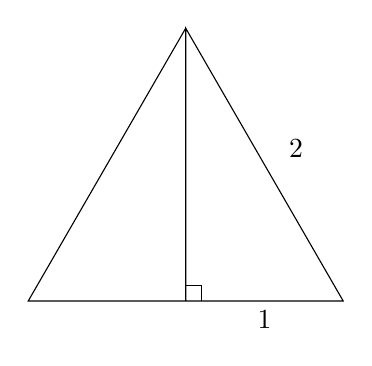
\begin{tikzpicture}[scale=2]
	\draw (0,0) -- (2,0) -- (1, 1.732050808) -- (1,0) -- (0,0) -- (1,1.732050808);
	\draw (1,.1) -- (1.1,.1) -- (1.1,0);
	\node at (1.5,0) [anchor=north] {1};
	\node at (1.7,.85) [anchor=south]{2};
\end{tikzpicture}
\caption{Special triangles are halves of thoroughly understood shapes.}
\end{center}
\end{figure}

According to the Pythagorean Theorem, what must the length of the 
hypotenuse be?  For either one of the triangles, what are the angles and
the ratios of the sides?

Next, consider an equilateral triangle with side of length 2.  If all the angles
are the same, what must they be?  Now we draw the perpendicular bisector,
which is also the altitude.  How long are the two half of the side we 
bifurcated?  What are the angles we split in two?  What would Pythagorus
tell you the length of the altitude is?

\begin{derivation}{Special Triangles}
The special triangles are derived from
squares and equilateral triangles.

A $45^\circ$-$45^\circ$-$90^\circ$ triangle has sides with ratios $1:1:\sqrt{2}$.

A $30^\circ$-$60^\circ$-$90^\circ$ triangle has sides with ratios $1:\sqrt{3}:2$.
\end{derivation}

Armed with such triangles, we can answer what sine, cosine, and tangent are
for $30^\circ$, $45^\circ$, and $60^\circ$, nine facts you should memorize.

\subsection{Reflection and Symmetry}
In the previous section of this chapter, we computed reference angles without
explaining why.  We will rectify that now.  Consider that there is a point $(x,y)$
somewhere in the first quadrant.  Draw a ray from the origin through this point,
and make it the terminal side of an angle.  Call that angle $\theta$.

\begin{figure}[h]
\begin{centering}
\begin{tikzpicture}[scale=0.5]
	\draw[<->, thick] (-4,0) -- (4,0);
	\draw[<->, thick] (0,-4) -- (0,4);
	\draw[fill] (55:3) circle (0.1) node[anchor=south] {$(x,y)$};
	\draw (3,0) arc(0:55:3);
	\node at (1,0.7) {$\theta$};
	\draw (0,0) -- (55:3);
\end{tikzpicture}
\caption{Turning angle $\theta$ results in going to coordinates $(x,y)$.}
\end{centering}
\end{figure}

What will be at the reference angle in the fourth quadrant?  If we turn
down from $0^\circ$ to $360^\circ-\theta$, we will be taken to $(x,-y)$.
In the second quadrant, the reference angle is $1800^\circ-\theta$, which
ends in the coordinates $(-x,y)$.  Finally, the third quadrant reference
angle of $180^\circ+\theta$ points to $(-x,-y)$.

Through the use of symmetry and reference angle, every fact we
learn in the first quadrant instantly reveals three other facts around
the grid.  Fill knowledge of the first quadrant entails full knowledge
of the entire Cartesian plane.

\begin{figure}[h]
\begin{centering}
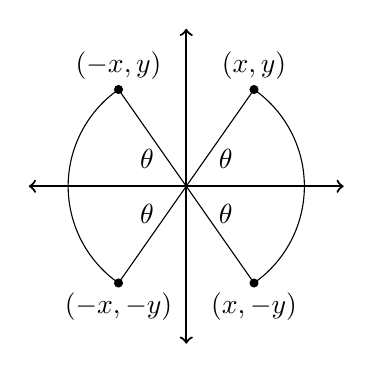
\begin{tikzpicture}[scale=0.5]
	\draw[<->, thick] (-4,0) -- (4,0);
	\draw[<->, thick] (0,-4) -- (0,4);
	
	\draw[fill] (55:3) circle (0.1) node[anchor=south] {$(x,y)$};
	\draw (3,0) arc(0:55:3);
	\node at (1,0.7) {$\theta$};
	\draw (0,0) -- (55:3);

	\draw[fill] (125:3) circle (0.1) node[anchor=south] {$(-x,y)$};
	\draw (0,0) ++ (125:3) arc(125:180:3);
	\node at (-1,0.7) {$\theta$};
	\draw (0,0) -- (125:3);

	\draw[fill] (235:3) circle (0.1) node[anchor=north] {$(-x,-y)$};
	\draw (0,0) ++ (180:3) arc(180:235:3);
	\node at (-1,-0.7) {$\theta$};
	\draw (0,0) -- (235:3);

	\draw[fill] (-55:3) circle (0.1) node[anchor=north] {$(x,-y)$};
	\draw (3,0) arc(0:-55:3);
	\node at (1,-0.7) {$\theta$};
	\draw (0,0) -- (-55:3);
\end{tikzpicture}
\caption{Reference angles are examples of horizontal and/or vertical symmetry. }
\end{centering}
\end{figure}


\subsection{$x$ and $y$ and slope}
Even the infinite number of points in the first quadrant can be scaled
down somewhat.  Let us consider only the points 1 unit away from
the origin.  Such points make a circle, called the Unit Circle.
If you think of sine as opposite over hypotenuse, and the hypotenuse is 
always 1, then on the unit circle, sine equals the opposite leg
of the reference triangle.  On the unit circle, this is always the $y$
value.  Sine \emph{is} $y$.

Again, if cosine is adjacent over hypotenuse and the hypotenuse is 
always one, then on the unit circle, cosine equals the adjacent leg
of the reference triangle.  On the unit circle, this always the $x$
value.  Cosine \emph{is} $x$.

Lastly, if tangent is opposite over adjacent, then on the unit circle
that is $y$ over $x$, rise over run, a.k.a. slope.  Tangent \emph{is}
slope.  And for any radius greater or less than 1, we need only 
multiply by that radius.  

When we overlay this way of thinking about trigonometric functions
(cosine is $x$, sine is $y$, tangent is slope) onto the grid, we can see
that all the first quadrant information we might gather can be
applied to any other quadrant with only sign changes.  Sine (as $y$)
will be positive in the first and second quadrant, and negative in
the third and fourth.  Cosine (as $x$) will be positive in the first
and fourth quadrants, and negative in the second and third.
Tangent (as $m$) will be positive in the first and third, and negative
in the second and fourth.

